\documentclass{beamer}
\usetheme[subsectionpage=progressbar, background=white]{metropolis}
\usepackage[utf8]{inputenc}
\usepackage{graphicx,color}
\usepackage{amsfonts}
\usepackage{amsmath}
\usepackage{amssymb}
\usepackage{verbatim}
\usepackage{fancyhdr}
\usepackage{epigraph}
\usepackage{caption}
\usepackage{psfrag}
\usepackage{afterpage}
\usepackage[backend=biber, style=nature]{biblatex}
\addbibresource{../bibTex/thesis-library.bib}
\useinnertheme{circles}
\graphicspath{{../figures/}}
%\setbeamercovered{transparent}
\newcommand{\Note}[1]{{\bf \color{red}#1}}    %Anotaciones
\newcommand{\esc}{\!\cdot\!}
\newcommand{\llangle}{\left\langle}
\newcommand{\rrangle}{\right\rangle}
\newcommand{\llg}{\left\lgroup}
\newcommand{\rlg}{\right\rgroup}
\newcommand{\bra}{\llbracket}
\newcommand{\ket}{\rrbracket}
\newcommand{\cc}{\!\parallel\!}
\newcommand{\GK}[2]{\langle#1 \cc #2\rangle}
\newcommand{\GKrest}[2]{\langle#1 \cc #2\rangle^0}

\title{Nanoscale hydrodynamics near solids}
\date{July 2019}
\author{Diego Duque Zumajo}
\institute{Departamento Física Fundamental \\Universidad Nacional de Educación a Distancia}

% logo of my university
\titlegraphic{%
\begin{picture}(0,0)
\put(308,-119){\makebox(0,0)[rt]{
\includegraphics[width=1.5cm]{logo}}}
\end{picture}}

\begin{document}
\maketitle

\begin{frame}{Motivation}
  \begin{itemize}
    \item Great interest in the study of fluids in contact with solids in the nanoscale.
        \item Density layering $\rightarrow$ DFT for equilibrium situations $\rightarrow$ DDFT for the study of the dynamic behaviour of the fluid. 
        \item Slip boundary condition
          \begin{align}
            \delta\frac{\partial v}{\partial z}=v_{\rm slip}, && \delta =\frac{\eta}{\gamma} \nonumber
          \end{align}
        \item Bocquet and Barrat \cite{Bocquet1993}
\begin{align}
  \gamma=\frac{1}{Sk_BT}\int_0^{\tau} dt \llangle \hat{F}^x(t)\hat{F}^x\rrangle
\nonumber
\end{align}
      \item Petravic and Harrowell \cite{Petravic2007} disagree with the expression obtained by Bocquet and Barrat.
      \item The expression for $\gamma$ suffers from the plateau problem. 
    \end{itemize}
\end{frame}

\begin{frame}{Roadmap}
  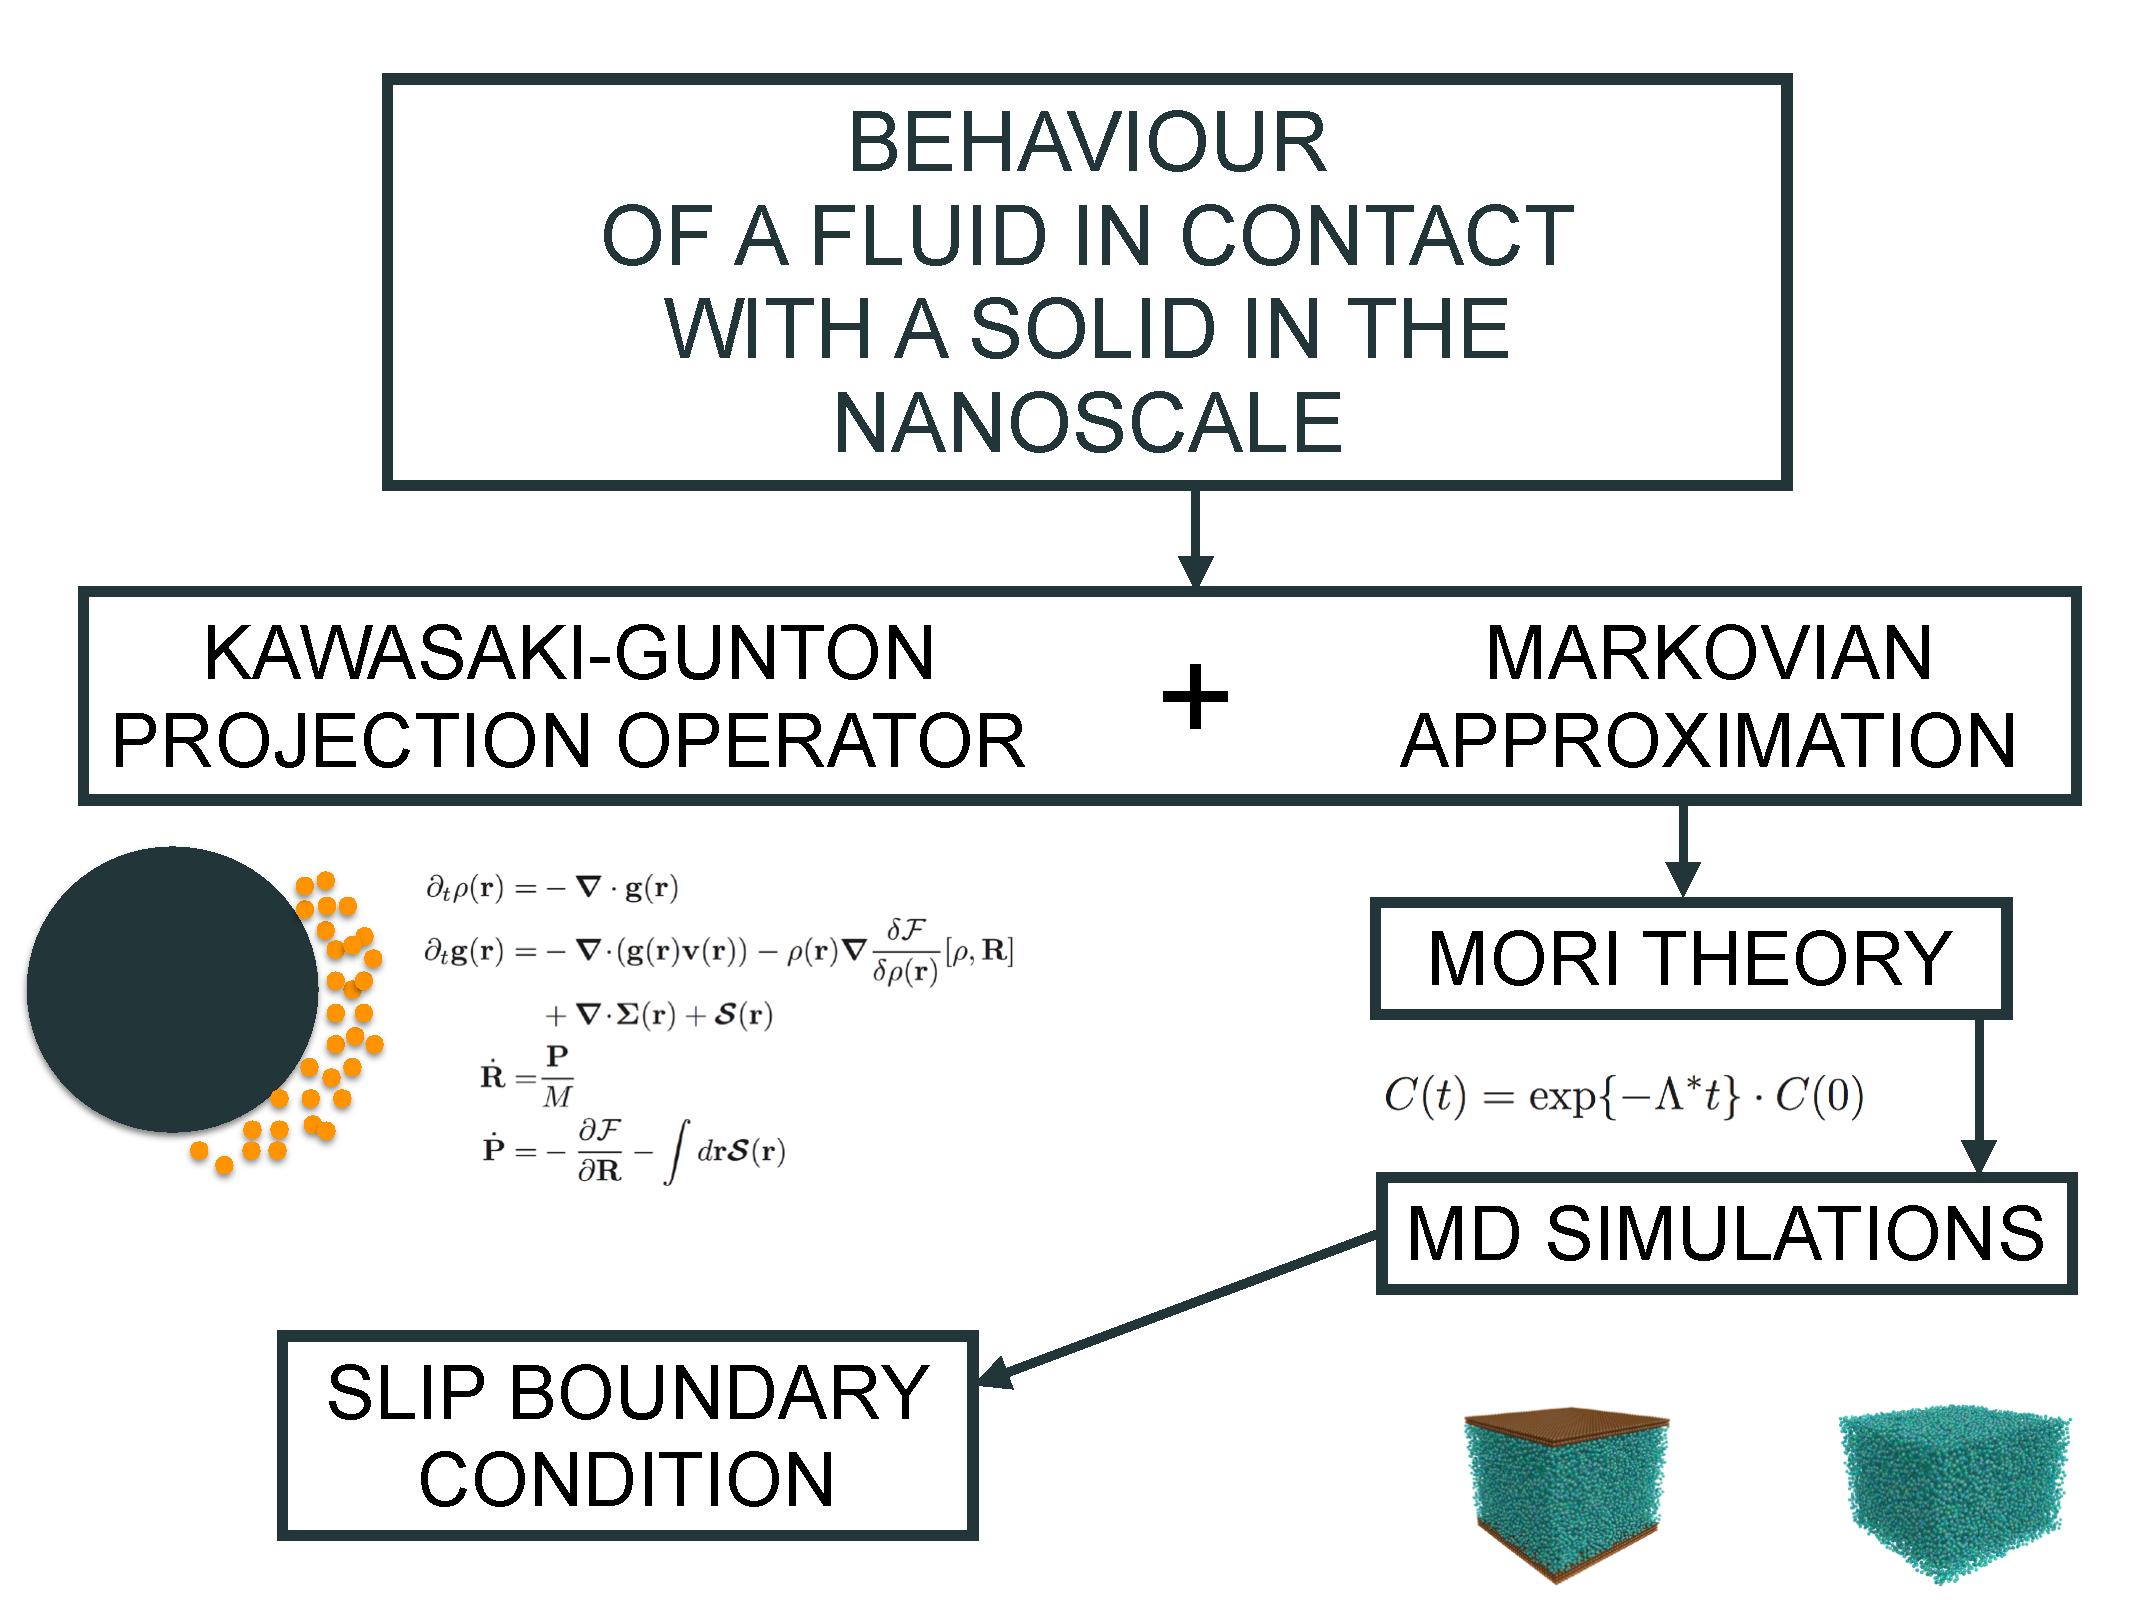
\includegraphics[width=\linewidth]{scheme-thesis}
\end{frame}

\section{Hydrodynamics theory for liquids near solids}
\begin{frame}{The system and the relevant variables}
  \begin{itemize}
    \item We study a fluid with $N$ particles in contact with a solid sphere of $N'$ particles.
    \item $z= ({\bf q}_i, {\bf p}_i)$ and $z'= ({\bf q}_{i'}, {\bf p}_{i'})$
    \item The relevant variables 
      \begin{align}
        \hat{\rho}_{\bf r}(z) &=\sum^{N}_im\delta({\bf r}-{\bf q}_i)
      &&\hat{\bf R}(z)=\frac{1}{N'}\sum_{i'}^{N'}{\bf q}_{i'}
      \nonumber\\
        \hat{\bf g}_{\bf r}(z) &=\sum^{N}_i{\bf p}_i\delta({\bf r}-{\bf q}_i)
      &&\hat{\bf P}(z)=\sum_{i'}^{N'}{\bf p}_{i'}
      \nonumber
      \end{align}
    \item The derivatives of the relevant variables
      \begin{align}
        i{\cal L} \hat{\rho}_{\bf r}(z) &= -\boldsymbol{\nabla}\esc\hat{\bf g}_{\bf r}(z)
        && i{\cal L}\hat{\bf R}(z) =\frac{\hat{\bf P}(z)}{M}
      \nonumber\\
      i{\cal L}\hat{\bf g}_{\bf r}(z)
          &=-\boldsymbol{\nabla}\cdot \hat{\boldsymbol{\sigma}}_{\bf r}(z)+\hat{{\bf F}}^{\rm s\to l}_{\bf r}(z) 
        &&i{\cal L}\hat{\bf P}(z) =-\int  d{\bf r} \hat{\bf F}^{\rm s\to l}_{\bf r}(z)
         \nonumber
\end{align}
    \end{itemize}
\end{frame}

\begin{frame}{Kawasaki-Gunton projection operator}
  \begin{itemize}
     \item Clear separation of timescales between the evolution of the averages and the decay of the memory kernel 
\begin{equation}
  \frac{\partial}{\partial t}a_i(t) = {\color{blue} v_i(t)} {\color{red} +\sum_j D_{ij}(t) \lambda_j(t)}
\nonumber
\end{equation}
\item {\color{blue} Reversible term}: $v_i={\rm Tr}[\overline{\rho}_t i{\cal L}\hat{A}_i]$ 
\item The relevant ensemble: 
  \begin{equation}
  \overline{\rho}(z) = \frac{1}{Z[\lambda]} \rho_0\exp\{-\lambda\!\cdot\!\hat{A}(z)\}
  \nonumber
  \end{equation}
\item {\color{red} The  dissipative matrix}  is  given  by  the Green-Kubo  formula
\begin{equation}
D_{ij}(t)=\int_0^{\Delta t} dt'\left\langle 
{\cal Q}_t i{\cal L}\hat{A}_j\exp\{i{\cal L}t'\}{\cal Q}_t i{\cal L}\hat{A}_i
\right\rangle^{\lambda(t)}
\label{dij}
\nonumber
\end{equation}
\item The Kawasaki-Gunton projection operator is given by 
  \begin{align}
    {\cal Q}_{t'}\hat{F}(z) &= \hat{F}(z)- {\rm Tr}[\overline{\rho}_{t'} \hat{F}]
  -\sum_i(\hat{A}_i(z)-a_i(t'))\frac{\partial }{\partial a_i(t')}
  {\rm Tr}[\overline{\rho}_{t'} \hat{F}]
  \label{Q}
  \nonumber
  \end{align}
\end{itemize}
\end{frame}

\begin{frame}{Equations of nanohydrodynamics}
\begin{align}
  \partial_t\rho({\bf r})=&{\color{blue} -\boldsymbol{\nabla}\cdot{\bf g}({\bf r})}
\nonumber\\
\partial_t{\bf g}({\bf r})=&{\color{blue} -\boldsymbol{\nabla}\esc{\left({\bf g}({\bf r}){\bf v}({\bf r})\right)}
-\rho({\bf r})\boldsymbol{\nabla}\frac{\delta {\cal F}}{\delta\rho({\bf r})}[\rho,{\bf R}]}
{\color{red} +\boldsymbol{\nabla}\esc\boldsymbol{\Sigma}({\bf r})+\boldsymbol{{\cal S}}({\bf r})}
\nonumber\\
\dot{\bf R}=&{\color{blue} \frac{\bf P}{M}}
\nonumber\\
\dot{\bf P}=&{\color{blue} -\frac{\partial {\cal F}}{\partial {\bf R}}}
{\color{red} -\int d {{\bf r}}\boldsymbol{{\cal S}}({\bf r})}
\nonumber
\end{align}

\begin{itemize}
  \item ${\cal F}[\rho, {\bf R}]$: free energy density functional of a fluid in the presence of a solid sphere.
  \item $\Sigma({\bf r})$: fluid stress tensor.
  \item ${\cal S}({\bf r})$: irreversible surface force density on the fluid.
\end{itemize}
\end{frame}

\begin{frame}{The transport kernels}
  \begin{itemize}
    \item The fluid stress tensor ${\color{red} \Sigma({\bf r})}$ is given by 
  \begin{align}
  \boldsymbol{\Sigma}^{\alpha\beta}({\bf r})&=
\int d{\bf r}'
\boldsymbol{\eta}^{\alpha\beta\alpha'\beta'}_{{\bf r}{\bf r}'}
\boldsymbol{\nabla}_{{\bf r}'}^{\beta'}{\bf v}^{\alpha'}({\bf r}')
\nonumber
\end{align}
\item The irreversible surface force density on the fluid ${\color{red} {\cal S}({\bf r})}$
\begin{align}
  \boldsymbol{{\cal S}}^\alpha({\bf r})=&
-\int d{\bf r}'{\bf G}^{\alpha\alpha'\beta'}_{{\bf r}{\bf r}'}
\boldsymbol{\nabla}_{{\bf r}'}^{\beta'} {\bf v}^{\alpha'}({\bf r}')
+\boldsymbol{\nabla}_{{\bf r}}^{\beta}\int d{\bf r}'{\bf H}^{\alpha\beta\alpha'}_{{\bf r}{\bf r}'}
( {\bf v}^{\alpha'}({\bf r}')-{\bf V}^{\alpha'})
\nonumber\\
&-\int d{\bf r}'
\boldsymbol{\gamma}^{\alpha\alpha'}_{{\bf r}{\bf r}'}( {\bf v}^{\alpha'}({\bf r}')
-{\bf V}^{\alpha'})
\nonumber
\end{align}
\end{itemize}
\end{frame}

\begin{frame}{The transport kernels}
\begin{align}
  \boldsymbol{\eta}_{{\bf  r}{\bf r}'} &\equiv
\frac{1}{k_BT}\int_0^{\Delta t} dt'\langle 
{\cal Q}_t\hat{\boldsymbol{\sigma}}_{{\bf r}}(t')
{\cal Q}_t\hat{\boldsymbol{\sigma}}_{{\bf r}'}\rangle^{\lambda(t)}
\nonumber \\
{\bf H}_{{\bf r}{\bf r}'}&\equiv\frac{1}{k_BT}\int_0^{\Delta t} dt'
\langle {\cal Q}_t\hat{\boldsymbol{\sigma}}_{{\bf r}}(t')
{\cal Q}_t\hat{\bf F}^{\rm s\to l}_{{\bf r}'}\rangle^{\lambda(t)}
\nonumber\\
{\bf G}_{{\bf r}{\bf r}'}&\equiv\frac{1}{k_BT}\int_0^{\Delta t} dt'
\langle {\cal Q}_t\hat{\bf F}^{\rm s\to l}_{{\bf r}}(t')
{\cal Q}_t\hat{\boldsymbol{\sigma}}_{{\bf r}'}\rangle^{\lambda(t)}
\nonumber\\
\boldsymbol{\gamma}_{{\bf  r}{\bf r}'}&\equiv\frac{1}{k_BT}\int_0^{\Delta t} dt'
\langle 
{\cal Q}_t\hat{\bf F}^{\rm s\to l}_{{\bf r}}(t')
{\cal Q}_t\hat{\bf F}^{\rm s\to l}_{{\bf r}'}\rangle^{\lambda(t)}
\nonumber
\end{align}
\end{frame}

\begin{frame}{Simpler theory}
  \begin{itemize}
    \item The amount of information to compute the hydrodynamic equations is exceedingly large:
      \begin{itemize}
        \item $\eta$ has 36 independent components. 
        \item ${\bf G}$ and ${\bf H}$ have 21 independent components. 
        \item $\gamma$ has 9 independent components. 
      \end{itemize}
    \item  The interactions felt by the fluid due to the walls are statistically planar and isotropic. We restric ourselves to planar flows. 
    \item In order to compare the hydrodynamic equations with the MD simulations we need a discrete version of the theory. 
    \end{itemize}
\end{frame}

\begin{frame}{Discrete basis function}
  \begin{itemize}
    \item $N_{\rm bin}$ bins with dimensions $L_x$, $L_y$, $\Delta z$ ($L_z/N_{\rm bin}$). 
      \begin{center}
        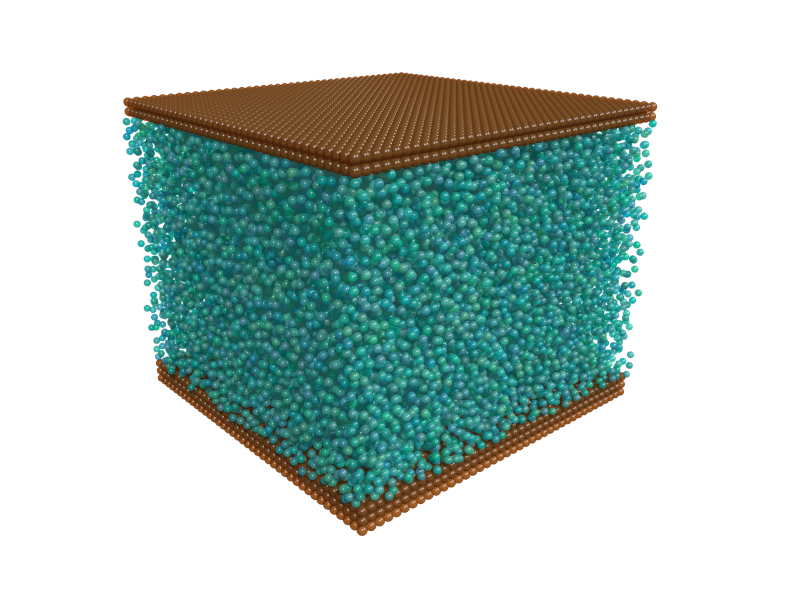
\includegraphics[width=.3\linewidth]{PRL3_gold2_wo_layers_wo_diffuse}
        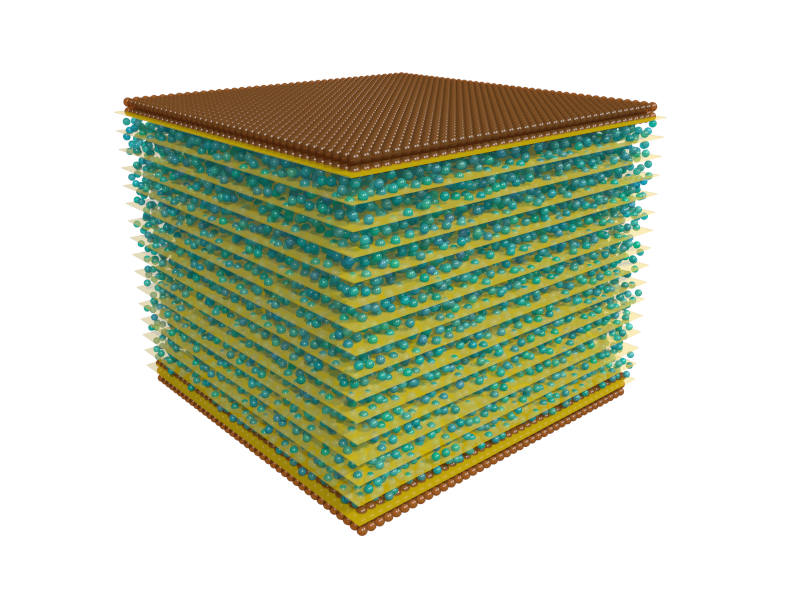
\includegraphics[width=.3\linewidth]{PRL3_gold2_wo_diffuse}
      \end{center}
    \item  Characteristic function $\chi_{\mu}({\bf r})$ and finite element linear basis function $\Phi_{\mu}({\bf r})$
    \begin{align}
    \chi_\mu({\bf r})&=\theta(z_{\mu+ 1}-z)\theta(z-z_\mu)=\chi_\mu(z)
    \nonumber
    \end{align}
    \begin{align}
      \Phi_\mu({\bf r})=\chi_\mu(z)\frac{z_{\mu+1}-z}{\Delta z}+\chi_{\mu-1}(z)\frac{z-z_{\mu-1}}{\Delta z}
      \nonumber
    \end{align}
    \begin{center} 
      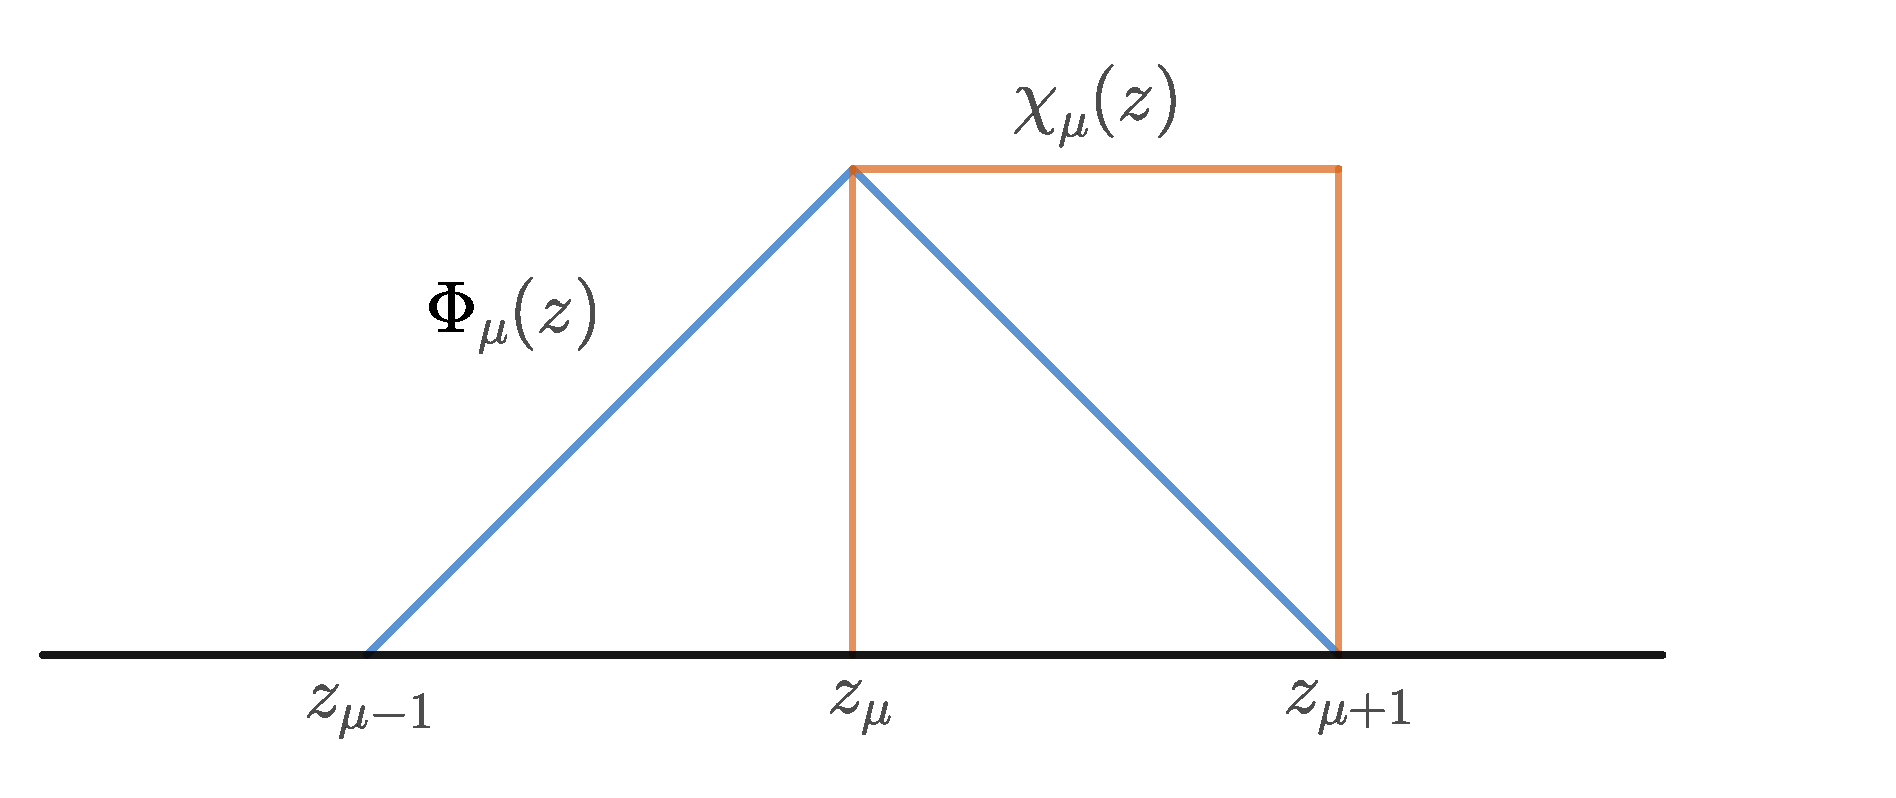
\includegraphics[scale=0.16]{psichi}
    \end{center}
  \end{itemize}
\end{frame}

\begin{frame}{Mass matrix and dual basis functions}
  \begin{itemize}
    \item The usual mass matrix of the finite element method is
      \begin{align}
      M^\Phi_{\mu\nu}&=\llg\Phi_\mu\Phi_\nu\rlg  
      \nonumber
      \end{align}
    \item We introduce the discrete velocity field in terms of $M^\Phi_{\mu\nu}$
      \begin{align}
        \tilde{{\bf v}}_{\mu}=\sum_{\nu}{\cal V}_{\mu}[M^{\Phi}]^{-1}_{\mu\nu}{\bf v}_{\nu}
        \nonumber
      \end{align}
  \item We can contruct continuum and discrete fields from dual basis functions $\delta_{\mu}({\bf r})$ and $\psi_\mu({\bf r})$ 
    \begin{align}
      v_\mu=\int d{\bf r}v({\bf r})\delta_\mu({\bf r}),&&
        \overline{v}({\bf r}) =\sum_{\mu}v_\mu\psi_\mu({\bf r})
    \nonumber
    \end{align}
  \end{itemize}
\end{frame}

\begin{frame}{Discrete equations of nanohydrodynamics}
\begin{align}
  \frac{d}{dt}\rho_\mu&=  {\color{blue} \llg\overline{\rho} \; \overline{\bf v}\boldsymbol{\nabla}\delta_\mu \rlg}
\nonumber\\
\frac{d}{dt}{\bf g}_\mu&=
{\color{blue} \llg\overline{\rho} \overline{\bf v}\;\overline{\bf v}\esc\boldsymbol{\nabla}\delta_{\mu}\rlg
-\sum_\nu\llg\overline{\rho}\delta_{\mu}\boldsymbol{\nabla}\delta_{\nu}\rlg
\frac{\partial  F}{\partial \rho_{\nu}}(\rho)}
\nonumber\\
&{\color{red}-\sum_{\nu}{\cal V}_\nu \frac{{\bf n}\esc\left[\boldsymbol{\eta}_{\mu\nu}-\boldsymbol{\eta}_{\mu-1\nu}-\boldsymbol{\eta}_{\mu\nu-1}+\boldsymbol{\eta}_{\mu-1\nu-1}\right]}{\Delta z^2}:{\bf n}\tilde{\bf v}_\nu}
\nonumber\\
&{\color{red}+\sum_{\nu}{\cal V}_\nu\frac{\left[{\bf G}_{\mu\nu}-{\bf G}_{\mu\nu-1}\right]}{\Delta z}\esc{\bf n}\tilde{\bf v}_\nu}
\nonumber\\
&{\color{red}+\sum_{\nu}{\cal V}_\nu\frac{{\bf n}\esc\left[{\bf H}_{\mu\nu}-{\bf H}_{\mu-1\nu}\right]}{\Delta z}\esc\tilde{\bf v}_\nu}
\nonumber\\
&{\color{red}-\sum_{\nu}{\cal V}_\nu\boldsymbol{\gamma}_{\mu\nu}\esc\tilde{\bf v}_\nu}
\nonumber
\end{align}
\end{frame}

\end{document}
